\documentclass[final]{siamltex}

\usepackage{graphicx}
\usepackage{subfigure}
\usepackage[colorlinks,unicode,linkcolor=black]{hyperref}
\usepackage{listings}
\lstset{
    language=C++,
    basicstyle=\small,
    columns=flexible,
    showstringspaces=false,
    numbers=left,
    numberstyle=\tiny,
    frame=leftline
    }

\newcommand{\code}[1]{\lstinline|#1|}
\newcommand{\figref}[1]{Fig.~\ref{#1}}
\newcommand{\eqref}[1]{(\ref{#1})}

%
% mathematical commands
%
\newcommand {\de} {\mbox{d}}
\newcommand {\ii} {\mathop{i}}
\newcommand {\rem}[1]{}

\title{Programming OpenCL and CUDA:\\a Case Study Using Modern C++ Libraries}

\author{
Karsten Ahnert\thanks{Institut f\"ur Physik und Astronomie, Universit\"at Potsdam,
Karl-Liebknecht-Strasse 24/25, 14476 Potsdam-Golm, Germany ({\tt
karsten.ahnert@gmx.de}) }
\and Denis Demidov\thanks{
Kazan Branch of Joint Supercomputer Center,
Russian Academy of Sciences,
Lobachevsky st. 2/31, 420008 Kazan, Russia
({\tt ddemidov@ksu.ru}) }
\and Karl Rupp\thanks{Mathematics and Computer Science Division,
Argonne National Laboratory,
9700 South Cass Avenue, Argonne, IL 60439, USA
({\tt rupp@iue.tuwien.ac.at}) } }

\begin{document}

\maketitle

\begin{abstract}
    We present a comparison of several modern C++ libraries intended for OpenCL
    and CUDA programming. The comparison is based on odeint, a framework for
    the solution of ordinary differential equations. Odeint is designed in a
    very flexible way and may be easily adapted for effective use of libraries such
    as VexCL, ViennaCL, or Thrust to solve ODEs with either OpenCL or CUDA
    technologies. We found that OpenCL and CUDA work equally well for problems
    of large sizes, while OpenCL has higher overhead for smaller problems.
    Furthermore, we show that modern high level libraries allow to effectively
    use computational resources of manycore GPUs or multicore CPUs without much
    knowledge of the underlying technologies.
\end{abstract}

\begin{keywords}
    GPGPU, OpenCL, CUDA, Modern C++ libraries, odeint, VexCL, ViennaCL, Thrust
\end{keywords}

\begin{AMS}
15A15, 15A09, 15A23
\end{AMS}


%
% INTRODUCTION
%
\section{Introduction}

\pagestyle{myheadings}

\thispagestyle{plain}
\markboth{K.~AHNERT, D.~DEMIDOV, AND K.~RUPP}{PROGRAMMING CUDA AND OPENCL\ldots}


Recently, general purpose computing on graphics processing units (GPGPU) has
acquired considerable momentum in the scientific community. This is confirmed
both by increasing numbers of GPGPU-related publications and GPU based
supercomputers in the Top 500\footnote{ \href{ http://top500.org }{
http://top500.org }} list. Major programming frameworks are NVIDIA CUDA and
OpenCL.  The former is a proprietary parallel computing architecture developed
by NVIDIA for general purpose computing on NVIDIA graphics adapters, and the
latter is an open, royalty-free standard for cross-platform, parallel
programming of modern processors maintained by the Khronos group. By nature,
the two frameworks have their distinctive pros and cons. CUDA has a more mature
programming environment with larger set of scientific libraries; but it is only
supported on NVIDIA hardware. OpenCL is supported on wide range of hardware,
but its native API requires much larger amount of boilerplate code from a
developer.

Both technologies are able to provide scientists with the vast computational
resources of modern GPU cards at the price of a steep learning curve.
Programmers need to familiarize
themselves with a new programming language and, more importantly, with a
new programming paradigm. However, the entry price may be lowered with help of
specialized libraries. The CUDA Toolkit includes several such libraries (BLAS
implementation, Fast Fourier Transform, Thrust and others). OpenCL lacks
standard libraries, but there are a number of third-party projects aimed at
developing both CUDA and OpenCL programs.

This paper presents comparison of several modern C++ libraries aimed
at ease of GPGPU development. We look at both convenience and
performance of the libraries under consideration in the context of
solving ordinary differential equations.  The comparison is based on
odeint, modern C++ library for solution of ODEs that has been recently
included into the Boost libraries\footnote{ \href{ http://boost.org }
  { http://boost.org } }.  The GPGPU libraries considered in this work
are Thrust, VexCL, and ViennaCL:

% [KR]: We need to define the scope of this work. We are investigating ODEs
% only, which we have to clarify.  There is a lot of GPGPU for dense linear
% algebra, sparse solvers, and molecular dynamics approaches. We don't consider
% any of these.

% [DD]: Is `the context of solving ordinary differential equations` not enough
% for this purpose? Or should we explicitly state that we are not intersted in
% the topics you mentioned?

\begin{description}
    \item[Odeint] is a modern C++ library\footnote{ \href{ http://odeint.com }{
	http://odeint.com } } for numerically solving Ordinary Differential
	Equations \cite{OdeintRef1, OdeintRef2}. It is developed in a generic
	way using Template Metaprogramming which leads to extraordinary high
	flexibility at top performance. The numerical algorithms are
	implemented independently of the underlying arithmetics. This results
	in a broad applicability of the library, especially in non-standard
	environments.  For example, odeint supports matrix types, arbitrary
	precision arithmetics and can be easily adopted to use either CUDA or
	OpenCL frameworks.  Odeint is used in this work as a framework for
	comparison of other libraries.
    \item[Thrust] is a parallel algorithms library\footnote{ \href{
	http://thrust.github.com }{ http://thrust.github.com }} which resembles
	the C++ Standard Template Library \cite{ThrustRef}.  Thrust's
	high-level interface greatly enhances developer productivity while
	enabling performance portability between GPUs and multicore CPUs.
	Thrust is distributed with NVIDIA CUDA Toolkit since version 4.1.
    \item[VexCL] is vector expression template
	library\footnote{ \href{ https://github.com/ddemidov/vexcl }{
	https://github.com/ddemidov/vexcl }} for OpenCL \cite{VexCLRef}. It has
	been created for ease of OpenCL development with C++.  VexCL strives to
	reduce the amount of boilerplate code needed to develop OpenCL
	applications. The library provides a convenient and intuitive notation
	for vector arithmetic, reduction, and sparse matrix-vector
	multiplication.  Multi-device and even multi-platform computations are
	supported.
    \item[ViennaCL] (The Vienna Computing Library) is a scientific computing
	library\footnote{ \href{ http://viennacl.sourceforge.net }{
	http://viennacl.sourceforge.net }} written in C++ and based on OpenCL
	\cite{ViennaCLRef}. It allows simple, high-level access to the vast
	computing resources available on parallel architectures such as GPUs
	and is primarily focused on common linear algebra operations (BLAS
	levels 1, 2 and 3) and the solution of large systems of equations by
	means of iterative methods with optional preconditioner.
\end{description}

CUDA and OpenCL differ in their handling of compute kernels compilation. In
NVIDIA's framework the compute kernels are compiled to PTX code together with
the host program. The PTX is pseudo-assembler language which is compiled at
runtime for the specific NVIDIA device it is being run on. Since PTX is already
very low-level, this just-in-time kernel compilation has low overhead. In
OpenCL the compute kernels are compiled at runtime from high level sources.
This adds an overhead which is particularly noticeable for smaller sized
problems. The pre-compilation to some low-level pseudo-code is not feasible in
OpenCL because it has to support wide range of hardware.

The approach to generation and compilation of the compute kernels is one of the
main differences between the OpenCL libraries we considered.  ViennaCL has
limited set of predefined kernels, which functionally coincides with BLAS level
1 routines.  These kernels are compiled in batch at the program start to allow
for faster initialization. However, due to this design decision each vector
expression may result in launch of more than one kernel.  On the other hand,
VexCL generates and compiles an OpenCL program with a single kernel for each
vector expression it encounters.  This leads to potentially higher
initialization overhead, but should prove to be more effective in the long
runs. It should be noted that main aim of ViennaCL is provision of iterative
solvers for large sparse systems of equations. In this context complex vector
expressions are rare and we believe that authors of ViennaCL made correct
design decision.  However, we think it is interesting to compare approaches of
VexCL and ViennaCL.

The other difference between CUDA and OpenCL is that CUDA supports subset of
C++ language in compute kernels, while OpenCL kernels are written in subset of
C99. Therefore, CUDA programmers may use template metaprogramming techniques
which may lead to more efficient and compact code.  Native OpenCL API does not
provide this feature, but the drawback is balanced by the ability for
on-the-fly kernel generation. Modern C++ libraries such as those considered in
this work successfully use this approach and hide gory details from their
users.




%
% ADAPTING ODEINT
%
\section{Adapting odeint}

Ordinary differential equations play a major role in many scientific
disciplines. They occur naturally in the context of mechanical
systems, like granular and molecular dynamics~--- in fact the Newtonian
and Hamiltonian mechanics are formulated as ordinary differential
equations. Many other applications can be found in such diverse
fields as biology and neuroscience, chemistry, social sciences, in
nonlinear science. Furthermore, ODEs are used to solve partial
differential equations (PDEs) numerically, they occur by discretization of
the spatial coordinates.

Odeint usually solves the initial value problem (IVP) of ordinary differential
equations.
\begin{equation}
\frac{\de x}{\de t } = \dot{x} = f(x , t), \quad \quad x(0) =
x_0.
\label{eq:ode}
\end{equation}
Here, $x$ is the dependent variable. It is usually a vector of real
values but also complex values are allowed. $t$ is the independent
variable. We will call $t$ the time throughout the article and we will
denote the time derivative with $\de x / \de t = \dot{x}$. $f(x,t)$ is
the system function and defines the ODE.

Numerous methods on solving ODEs exist \cite{HairerSolvingODEI,
  HairerSolvingODEII, HairerGeometricNumericalIntegration2006}. They
are usually categorized in the field of numerical analysis. Odeint
implements the most prominent of these methods, for example the
classical Runge-Kutta methods and Runge-Kutta-Fehlberg methods,
multistep methods (Adams-Bashforth-Moulton), symplectic
Runge-Kutta-Nystr\"om methods, and implicit methods (Rosenbrock and
implicit Euler). All of these methods work iteratively. They start
from a given initial value $x(t_0)$ to calculate the next value
$x(t+\Delta t)$. $\Delta t$ is the step size. This value acts then as
the starting value for the next iteration and so. The most simple
method one can imagine is the explicit Euler scheme
\begin{equation}
x\left(t+\Delta t\right) = x(t) + \Delta t \; f(x(t),t).
\label{eq:euler}
\end{equation}
It is usually not used for real applications but is used here for
demonstration purposes. The accuracy of the Euler scheme is not very
good and one needs to perform many steps with small step size to
obtain reasonable results.


One main feature of odeint is the decoupling of the specific algorithm
for solving the ODE from the underlying arithmetic operations. This
is achieved by a combination of a state type, an algebra and
operations. The state type represents the state of the ODE being
solved and is usually a vector type like \code{std::vector<>},
\code{std::array<>}, or a vector residing on a GPU. The algebra is
responsible for iterating through all elements of the state whereas
the operations are responsible for the elementary operations.

To see how this works consider an implementation of the Euler method.
% add a sentence about the Euler method, with the formula.
\begin{lstlisting}
template< class State, class Algebra, class Operations >
class euler {
    // ...
    template< class Ode >
    void do_step(Ode ode, State &x, time_type t, time_type dt) {
        ode(x, m_dxdt, dt);
        Algebra::for_each3( x, x, m_dxdt, Operations::scale_sum2(1.0, dt) );
    }
};
\end{lstlisting}
The state type, the algebra, and the operations enter the stepper as
template parameter, hence they are exchangeable. The function object
ode represents the ODE and must be provided by the user. It calculates
the r.h.s. of \eqref{eq:ode} and stores the result in
\code{m_dxdt}. The call of \code{for_each3} iterates three vectors and
applies on each element \code{scale_sum2}. The operation is performed
in-place, meaning that $x$ is updated to the new value. The main
reason for the separation here is that all arithmetic calculations and
iterations are completely encapsulated into the algebra and the
operations which must be provided by the user. Note, that algebra and
the operations must be chosen such that they interact correctly with
the state type.

% [KA]: Maybe the paragraph above explains the functioning a bit better.
% The paragraph is not finished and 
% it requires to put the paragraphs about ODEs in front of this paragraph.

% [DD]: I like it better than the paragraph below. That I took from odeint
% documentation and it feels out of context here. May be we should omit it.

Odeint provides a set of predefined algebras, which includes:
\begin{remunerate}
\item \code{range_algebra}: default algebra which works on Boost.Ranges;
\item \code{array_algebra}: specialized algebra for \code{boost::array};
\item \code{fusion_algebra}: algebra for compile-time sequences like
  \code{boost::fusion::vector}, \code{std::tuple}, etc.;
\item \code{vector_space_algebra}: algebra for vector space types that
  provide overloaded arithmetic operators for elementwise operations.
\end{remunerate}
Each of these algebras is a class consisting of \code{for_each1},
\dots, \code{for_eachN} methods. For example the \code{for_each3}
method in the \code{range_algebra} is similar to
\begin{lstlisting}
struct range_algebra {
    // ...
    template< class R1, class R2, class Op >
    void for_each2(R1 &r1, R2 &r2, Op op) {
        auto it1 = boost::begin(r1);
        auto it2 = boost::begin(r2);
        while(it1 != boost::end(r1)) op( *it1++, *it2++ );
    }
    // ...
};
\end{lstlisting}
The operations are represented by a struct with public member classes defining the
operations which are used by the algebras. There is only one default
operations class implementation in odeint
\begin{lstlisting}
struct default_algebra {
    // ...
    template< class Fac1, class Fac2 >
    struct scale_sum2 {
        Fac1 m_fac1;
        Fac2 m_fac2;
        scale_sum2( Fac1 fac1, Fac2 fac2 ) : m_fac1(fac1), m_fac2(fac2) { }
        template< class S1, class S2, class S3 >
        void operator()( S1 &s1, const S2 &s2, const S3 &s3 ) const {
            s1 = m_fac1 * s2 + m_fac2 * s3;
        }
    };
    // ...
};
\end{lstlisting}


Many libraries for vector and matrix types provide expression
templates for the elementary operations. Such libraries do not need an
own algebra but can be used with the \code{vector_space_algebra} and
the \code{default_operations} which simply calls the operations
directly on the matrix or vector type. In this case only odeint
resizing mechanism has to be adapted.

We describe odeint adaptation for GPGPU libraries under consideration
in the paragraphs below. We should mention that odeint now supports
all of the considered libraries natively. However, providing
adaptation examples serves our goal of comparing convenience of the
libraries interfaces.

To adapt Thrust to odeint we need to provide both an algebra and
operations. The algebra should define the \code{for_each} family of
algorithms. All of these operations look very similar to each other,
so we only provide \code{for_each3} code here:
\begin{lstlisting}
struct thrust_algebra {
    template<class StateType1, class StateType2, class StateType3, class Operation>
    static void for_each3(StateType1 &s1, StateType2 &s2, StateType3 &s3, Operation op)
    {
        thrust::for_each(
                thrust::make_zip_iterator( thrust::make_tuple(
		    boost::begin(s1), boost::begin(s2), boost::begin(s3) ) ),
		thrust::make_zip_iterator( thrust::make_tuple( 
		    boost::end(s1), boost::end(s2), boost::end(s3) ) ),
		op);
    }
};
\end{lstlisting}

The operations that are called in the \code{for_each} family of algorithms are
defined in \code{thrust_operations} and are actually device functors:
\begin{lstlisting}
struct thrust_operations {
    template<class Fac1 = double, class Fac2 = Fac1>
    struct scale_sum2 {
        const Fac1 m_alpha1;
        const Fac2 m_alpha2;

        scale_sum3(const Fac1 alpha1, const Fac2 alpha2)
	    : m_alpha1(alpha1), m_alpha2(alpha2) { }

        template< class Tuple >
        __host__ __device__ void operator()( Tuple t ) const {
            thrust::get<0>(t) = m_alpha1 * thrust::get<1>(t)
	                       + m_alpha2 * thrust::get<2>(t);
        }
    };
\end{lstlisting}

As you can see, \code{thrust::make_zip_iterator} is used here to pack several
device vectors into single iterable sequence. The sequence is then processed by
the \code{thrust::for_each} algorithm and the device functor which uses
\code{thrust::get<>} functions to unpack the zip iterator into separate values.
This approach is heavily used with Thrust and allows to process several vectors
in single efficient sweep. Adaptation of resizing operations is trivial and is
omitted here for the sake of conciseness.


Both VexCL and ViennaCL provide convenient expression templates that
may be directly used with odeint's \code{vector_space_algebra} and
\code{default_operations}. This combination proved to be 
effective with VexCL where each expression results in a single
kernel. For ViennaCL though default operations involving more than two
terms result in multiple kernel launches.  Moreover, temporary vectors
are allocated and deallocated for each of such composite operations.
This results in dramatic decrease of performance, so we had to provide
specialized operations for ViennaCL. These use a custom kernel
generation mechanism provided by the library.  For example,
\code{scale_sum2} operation is defined as:
\begin{lstlisting}
struct viennacl_operations {
    // ...
    template<class Fac1 = double, class Fac2 = Fac1>
    struct scale_sum2 {
	// ...
        template<class T1, class T2, class T3>
        void operator()( viennacl::vector<T1> &v1,
                const viennacl::vector<T2> &v2,
                const viennacl::vector<T3> &v3
                ) const
        {
            using namespace viennacl;

            static generator::symbolic_vector    <0, T1>   sym_v1;
            static generator::symbolic_vector    <1, T2>   sym_v2;
            static generator::symbolic_vector    <2, T3>   sym_v3;
            static generator::cpu_symbolic_scalar<3, Fac1> sym_a1;
            static generator::cpu_symbolic_scalar<4, Fac2> sym_a2;

            static generator::custom_operation op(
                    sym_v1 = sym_a1 * sym_v2
                           + sym_a2 * sym_v3,
		    "scale_sum2"
                    );

            ocl::enqueue( op(v1,
                        const_cast< vector<T2>& >(v2),
                        const_cast< vector<T3>& >(v3),
                        const_cast< Fac1& >(m_alpha1),
                        const_cast< Fac2& >(m_alpha2)
                        ) );
        }
    };
    // ...
};
\end{lstlisting}
Here custom kernel is automatically generated from symbolic vector expression
once and is called whenever the operation is required.  Resizing operations for
both of OpenCL libraries are trivial and not provided here.




\section{Numerical experiments}

Typical use cases for solving ODEs on GPUs are large systems of
coupled ODEs which occur as discretizations of PDEs, or in ODEs
defined on lattices or graphs. Another use case are parameter studies,
where one wants to study the dependence of an ODE on some
parameters. Here, one creates one large ODE which consists of many
small uncoupled ODEs, each with a different parameter set. This one
large system is then solved at once, hence all small ODEs are solved
simultaneously.

In this section we will show four examples and study their
performance. Two examples are of the first type, namely a
one-dimensional lattice of simple phase oscillators and a
two-dimensional Hamiltonian lattice. The other two examples are
parameter studies.






%
% DAMPED OSCILLATOR
%
\subsection{Damped Harmonic Oscillator Ensemble}

The first example is a set of damped driven oscillators
\begin{equation} \label{eq:dampedsystem}
    \dot{x} = \omega y + \varepsilon x, \quad \quad
    \dot{y} = -\omega x + \varepsilon y
\end{equation}
with $\varepsilon = \varepsilon_0 + \varepsilon_a \cos \left( \omega_d
t \right)$. $\omega$ is the natural frequency of the oscillator and
$\varepsilon$ is the time dependent damping constant.  Note, that this form is
not the classical form of a damped oscillator, but can be derived easily from
$\ii \dot{\Psi} = \omega \Psi + \ii \varepsilon \Psi$ with $\Psi = x + \ii y$.


The Thrust version of the system functor for the damped harmonic oscillator
ensemble example is presented below. The functor holds model parameters and
provides \code{operator()} with a signature required by the odeint library. The
state type is represented by \code{thrust::device_vector<double>}:
\begin{lstlisting}
typedef thrust::device_vector<double> state_type;

struct oscillator {
    size_t N;
    double omega, amp, offset, omega_d;

    oscillator(size_t N, double omega, double amp, double offset, double omega_d)
        : N(N), omega(omega), amp(amp), offset(offset), omega_d(omega_d) { }

    void operator()(const state_type &x, state_type &dxdt, double t) const;
};
\end{lstlisting}
$X$ and $Y$ components of the state are held in first and second halves of the
vector correspondingly.  \code{operator()} uses the standard technique of
packing the state components into a zip iterator and passes the composite
sequence to \code{thrust::for_each} algorithm together with the provided device
functor:
\begin{lstlisting}[firstnumber=12]
struct oscillator_functor;

void oscillator::operator()(const state_type &x, state_type &dxdt, double t) const {
    double eps = offset + amp * cos(omega_d * t);
    thrust::for_each(
        thrust::make_zip_iterator(
            thrust::make_tuple(
                boost::begin(x), boost::begin(x) + N,
                boost::begin(dxdt), boost::begin(dxdt) + N ) ),
        thrust::make_zip_iterator(
            thrust::make_tuple(
                boost::begin(x) + N, boost::end(x),
                boost::begin(dxdt) + N, boost::end(dxdt) ) ),
        oscillator_functor(omega, eps) );
}
\end{lstlisting}
The device functor unpacks individual components and applies the required
operations to the derivative part:
\begin{lstlisting}[firstnumber=last]
struct oscillator_functor {
    double eps, omega;

    oscillator_functor(double omega, double eps) : omega(omega), eps(eps) {}

    template< class T >
    __host__ __device__ void operator()(T t) const {
        double x = thrust::get< 0 >( t );
        double y = thrust::get< 1 >( t );
        thrust::get<2>(t) = eps * x + omega * y;
        thrust::get<3>(t) = eps * y - omega * x;
    }
};
\end{lstlisting}


The system functor for the VexCL version of the damped harmonic oscillator
example is much simpler than the Thrust variant because VexCL supports a rich
set of vector expressions. The state is represented by the
\code{vex::multivector<double,2>} type which holds two instances of
\code{vex::vector<double>} and transparently dispatches all operations to the
underlying components. The code for \code{operator()} body practically
coincides with the problem statement \eqref{eq:dampedsystem}:
\begin{lstlisting}
typedef vex::vector<double> vector_type;
typedef vex::multivector<double, 2> state_type;

struct oscillator {
    double omega, amp, offset, omega_d;

    oscillator(double omega, double amp, double offset, double omega_d)
        : omega(omega), amp(amp), offset(offset), omega_d(omega_d) { }

    void operator()(const state_type &x, state_type &dxdt, double t) const {
        double eps = offset + amp * cos(omega_d * t);
        dxdt(0) = eps * x(0) + omega * x(1);
        dxdt(1) = eps * x(1) - omega * x(0);
    }
};
\end{lstlisting}


The drawback of this variant is that it leads
to two kernel launches (one per each vector assignment) and results in
suboptimal performance. We are not able to use simple multivector arithmetic
operations here because components in the right hand sides of the assignments
are interchanged.  Fortunately, VexCL provides notation for such
multi-operations.  Assignment of a tuple of expressions to a multivector leads
to generation and launch of single efficient OpenCL kernel. This notation is
only slightly more cumbersome than the above variant:
\begin{lstlisting}[firstnumber=11]
double eps = offset + amp * cos(omega_d * t);
dxdt = std::make_tuple(     eps * x(0) + omega * x(1),
                            eps * x(1) - omega * x(0)   );
\end{lstlisting}

The ViennaCL version of the damped harmonic oscillator example uses
\code{boost::fusion::vector} to pack coordinate components of the state into a
single type. Individual components are instances of
\code{viennacl::vector<double>} type.

ViennaCL, as well as VexCL, supports expression templates for a limited set of
vector operations (closely corresponding to Level 1 BLAS routines). More
complex expressions may be built with help of the ViennaCL kernel generator
interface, which supports single- or multiple-operations kernels. The required
notation is a bit more cumbersome than that of VexCL library. OpenCL kernels
here are generated from symbolic expressions involving explicit symbolic types:
\begin{lstlisting}
typedef viennacl::vector<double> vector_type;
typedef fusion::vector<vector_type, vector_type> state_type;

struct oscillator {
    double omega, amp, offset, omega_d;

    viennacl::generator::symbolic_vector<0, double> sym_dx;
    viennacl::generator::symbolic_vector<1, double> sym_dy;
    viennacl::generator::symbolic_vector<2, double> sym_x;
    viennacl::generator::symbolic_vector<3, double> sym_y;
    viennacl::generator::cpu_symbolic_scalar<4, double> sym_eps;
    viennacl::generator::cpu_symbolic_scalar<5, double> sym_omega;
    viennacl::generator::custom_operation op;

    oscillator(double omega, double amp, double offset, double omega_d)
        : omega(omega), amp(amp), offset(offset), omega_d(omega_d),
          op(sym_dx = sym_eps * sym_x + sym_omega * sym_y,
             sym_dy = sym_eps * sym_y - sym_omega * sym_x,
             "oscillator")
    { }

    void operator()( const state_type &x, state_type &dxdt, double t );
};
\end{lstlisting}

This requires more of boilerplate code but the resulting expression tree
carries information of whether two terminals represent the same vector
instance. This in principle allows generation of more effective code. The
\code{operator()} unpacks \code{boost::fusion::vector} container and launches
the generated kernel:
\begin{lstlisting}[firstnumber=24]
void oscillator::operator()( const state_type &x, state_type &dxdt, double t ) {
    vector_type &X  = const_cast<vector_type&>( fusion::at_c<0>(x) );
    vector_type &Y  = const_cast<vector_type&>( fusion::at_c<1>(x) );
    vector_type &dX = fusion::at_c<0>(dxdt);
    vector_type &dY = fusion::at_c<1>(dxdt);

    double eps = offset + amp * cos(omega_d * t);
    viennacl::ocl::enqueue( op(dX, dY, X, Y, eps, omega) );
}
\end{lstlisting}




%
% PHASE OSCILLATORS
%
\subsection{Chain of Coupled Phase Oscillators}

As a second example we consider a chain of coupled phase
oscillators. A phase oscillator describes the dynamics of an
autonomous oscillator \cite{PhaseOscillator}. Its evolution is
governed by the phase, a $2\pi$ periodic variable which grows linearly
in time $\dot{\varphi} = \omega$, where $\omega$ is the phase
velocity. The amplitude of the oscillator does not occur in this
equation, so an interesting behaviour can only be observed if many
of such oscillators are coupled. In fact, such a system can be used to
study such divergent phenomena as synchronization, wave and pattern
formation, phase chaos, or oscillation death
\cite{Synchronization-Pikovsky,Kuramoto-84}. It is a prominent example
of an emergent system where the coupled system shows more complex
behaviour than its constitutes.


The concrete example we analyze here is a chain of nearest-neighbor
coupled phase oscillators:
\begin{equation} \label{eq:phasesystem}
    \dot{\varphi}_i = \omega_i + \sin( \varphi_{i+1} - \varphi_i) + \sin( \varphi_i
    - \varphi_{i-1}).
\end{equation}
The index $i$ denotes here the $i$-th phase in the chain. Note, that
the phase velocity is different for each oscillator.

The Thrust version for the coupled phase oscillator chain looks very similar to
the damped oscillator example. Again, we use a zip iterator to pack required
components and process the resulting sequence with single sweep of the
\code{for_each} algorithm. The only difference here is that we need values of
neighboring vector elements. In order to provide the values, we use Thrust's
permutation iterator, so that \code{operator()} of the system functor looks
like
\begin{lstlisting}
thrust::for_each(
    thrust::make_zip_iterator(
        thrust::make_tuple(
            x.begin(),
            thrust::make_permutation_iterator( x.begin(), prev.begin() ),
            thrust::make_permutation_iterator( x.begin(), next.begin() ),
            omega.begin(),
            dxdt.begin() ) ),
    thrust::make_zip_iterator(
        thrust::make_tuple(
            x.end(),
            thrust::make_permutation_iterator( x.begin(), prev.end() ),
            thrust::make_permutation_iterator( x.begin(), next.end() ),
            omega.end(),
            dxdt.end() ) ),
    sys_functor()
    );
\end{lstlisting}
\code{prev} and \code{next} are instances of
\code{thrust::device_vector<size_t>} holding indices to left and right vector
elements and initialized as
\begin{lstlisting}
thrust::counting_iterator<size_t> c(0);
thrust::copy(c, c + N - 1, prev.begin() + 1);
prev[0] = 0;     // prev = { 0, 0, 1, 2, 3, ..., N-1 }
thrust::copy(c + 1, c + N, next.begin());
next[N-1] = N-1; // next = { 1, 2, 3, ..., N-1, N-1 }
\end{lstlisting}

The VexCL version of the example is presented below.  Again, it is the most
concise variant since VexCL provides native support for the user-defined
stencils operations. The sum of sines in \eqref{eq:phasesystem} is encoded
using the \code{vex::StencilOperator<>} class template.  Template parameters
are the body string for the generated OpenCL function encoding required
operation, width and center point of the stencil, and its return type. Once the
stencil operator is defined, the functor's \code{operator()} is implemented
with a single line of code:
\begin{lstlisting}
typedef vex::vector<double> state_type;
extern const char oscillator_body[] = "return sin(X[-1] - X[0]) + sin(X[0] - X[1]);";

struct phase_oscillators {
    const state_type &omega;
    vex::StencilOperator< double, 3, 1, oscillator_body > S;
    phase_oscillators(const state_type &omega) : omega(omega), S(omega.queue_list()) { }
    void operator()(const state_type &x, state_type &dxdt, double t) const {
        dxdt = omega + S(x);
    }
};
\end{lstlisting}


ViennaCL, being oriented at iterative solution of large systems of equations,
does not provide stencil operations required for the problem at hand, so we had
to fallback to hand-coded OpenCL kernel:
\begin{lstlisting}
static const char phase_oscillator_source[] =
    "#pragma OPENCL EXTENSION cl_khr_fp64: enable\n"
    "kernel void oscillator(\n"
    "        uint n,\n"
    "        global double *dx,\n"
    "        global const double *x,\n"
    "        global const double *omega\n"
    "        )\n"
    "{\n"
    "    for(uint i = get_global_id(0); i < n; i += get_global_size(0)) {\n"
    "        double X0 = x[i];\n"
    "        double Xl = i > 0 ? x[i - 1] : X0;\n"
    "        double Xr = i + 1 < n ? x[i + 1] : X0;\n"
    "        dx[i] = omega[i] + sin(Xl - X0) + sin(X0 - Xr);\n"
    "    }\n"
    "}\n";
\end{lstlisting}
ViennaCL provide convenient mechanism for compilation and launching of custom
kernels, so this was a pleasant experience in comparison with native OpenCL
API. This low-level variant expectedly turned out to be the most effective one
(see the Results section):
\begin{lstlisting}[firstnumber=last]
typedef viennacl::vector<double> state_type;

struct phase_oscillators {
    const state_type &omega;
    sys_func(const state_type &omega) : omega(omega) {
        viennacl::ocl::current_context().add_program(phase_oscillator_source,
            "oscillator_program").add_kernel("oscillator");
    }
    void operator()(const state_type &x, state_type &dxdt, double t) const {
        viennacl::ocl::kernel &step = viennacl::ocl::current_context().get_program(
            "oscillator_program").get_kernel("oscillator");
        viennacl::ocl::enqueue( step(static_cast<cl_uint>(x.size()), dxdt, x, omega) );
    }
};
\end{lstlisting}








%
% DISORDERED LATTICES
%
\subsection{Disordered Hamiltonian Lattice}


Another example for our performance and usage study is a strongly
nonlinear disordered Hamiltonian lattice. Its equations of motion are
governed by
\begin{equation}
\dot{q}_{i,j} = p_{i,j}, \quad \quad 
\dot{p}_{i,j} = - \omega_{i,j}^2 q_i - \beta q_{i,j}^3 + \Delta_d q_{i,j}.
\label{eq:disordered_ham}
\end{equation}
Here, $\Delta_d q_{i,j}$ denotes the two-dimensional discreet Laplacian
$\Delta_d
q_{i,j}=q_{i+1,j}+q_{i-1,j}+q_{i,j+1}+q_{i,j-1}-4q_{i,j}$. Such
systems are widely used in theoretical physics to study phenomena
like Anderson localization or thermalization.

An important property of \eqref{eq:disordered_ham} is its Hamiltonian
nature. It can be obtained from Hamilton equations, and the energy and
phase volume are conserved during the time evolution. To account for
these properties, a special class of solvers exists, namely symplectic
solvers. Odeint implements three different variants of such solvers,
all are of the Runge-Kutta-Nystr\"om type.



The natural choice for the implementation of \eqref{eq:disordered_ham} is a
sparse matrix~-- vector product. Unfortunately, Thrust provides neither a sparse
matrix type, nor sparse matrix-vector product operation.  We had to combine
Thrust with the CUSPARSE library in order to implement this example. CUSPARSE
contains a set of basic linear algebra subroutines used for handling sparse
matrices and is included in CUDA Toolkit distribution as well as Thrust
library. Another possibility would be to use an open source Cusp library~--- a
library for sparse linear algebra and graph computations on CUDA
\cite{CuspRef}.

All of the libraries considered in our study use the hybrid
ELL format for storing the sparse matrix, which is one of the most efficient
formats for sparse matrices on GPUs~\cite{BellGarland2008}.

The linear combination $\Delta_d q_{i,j} - \omega^2_{i,j}q_i$ may be represented
as a single sparse matrix.  As the construction of the matrix is
straight-forward, we only provide code for the system functor's
\code{operator()}.

The Thrust version of the system functor looks like this:
\begin{lstlisting}
typedef thrust::device_vector<double> state_type;

void operator()(const state_type &q , state_type &dp) const {
    static double one = 1;
    thrust::transform(q.begin(), q.end(), dp.begin(), scaled_pow3_functor(-beta) );

    cusparseDhybmv(handle, CUSPARSE_OPERATION_NON_TRANSPOSE,
            &one, descr, A, thrust::raw_pointer_cast(&q[0]), &one,
            thrust::raw_pointer_cast(&dp[0]) );
}
\end{lstlisting}
Here \code{handle}, \code{descr}, and \code{A} are CUSPARSE data structures
holding CUSPARSE context and sparse matrix data. In lines 5 and 6
\code{thrust::transform()} algorithm is used to compute scaled cube of input
vector \code{q}. Lines 7--9 call procedure for sparse matrix~-- vector product.
Function \code{thrust::raw_pointer_cast()} is used to convert thrust device
vector iterator to raw device pointer.

The VexCL version employs the user-defined OpenCL function \code{pow3} which
computes the third power of its argument and is used for the performance sake.
\code{A} is \code{vex::SpMat<double>} instance holding discretization of linear
combination $\Delta_d q_{i,j} - \omega^2_{i,j}q_i$:
\begin{lstlisting}
typedef vex::vector<double> state_type;

extern const char pow3_body[] = "return prm1 * prm1 * prm1;";
vex::UserFunction<pow3_body, double(double)> pow3;

void ham_lattice::operator()(const state_type &q, state_type &dp) const {
    dp = (-beta) * pow3(q) + A * q;
}
\end{lstlisting}

ViennaCL neither supports elementwise vector product nor provides
overloaded math functions for its vector types. Therefore, we had to split its
\code{operator()} into two parts: the first part computes sparse matrix~--
vector product normally, while the second part uses a hand-coded kernel to
subtract non-linear term $\beta q^3$ from the result:
\begin{lstlisting}
typedef viennacl::vector<double> state_type;

void ham_lattice::operator()(const state_type &q, state_type &dp) const {
    dp = viennacl::linalg::prod(A, q);

    viennacl::ocl::kernel &scaled_pow3 =
        viennacl::ocl::current_context().get_program(
                "pow3_program").get_kernel("scaled_pow3");

    viennacl::ocl::enqueue(
        scaled_pow3(static_cast<cl_uint>(q.size()), dp, q, beta) );
}
\end{lstlisting}









%
% LORENZ ATTRACTOR, OPTIONAL
%
\subsection{Lorenz Attractor Ensemble}

In the fourth example we will use the Lorenz system \cite{Lorenz-63}. The
Lorenz system is a system of three coupled ODEs which shows chaotic
behavior for a large range of parameters. It is one of the most frequently
used ODE for evaluation purposes in the nonlinear dynamics community.
The ODE of the Lorenz system reads
\begin{equation}
  \dot{x} = -\sigma \left( x - y \right), \quad 
  \dot{y} = R x - y - xz, \quad
  \dot{z} = -bz + xy.
  \label{eq:lorenz}
\end{equation}


Solutions of the Lorenz system usually furnish a very interesting
behavior in dependence on one of its parameters.  For example, one
might want to study the dependence on the chaoticity on the parameter
$R$. Therefore, one would create a large set of Lorenz systems (each
with a different parameter $R$), pack them all into one system and
solve them simultaneously. (In a real study of chaoticity one would
usually calculate the Lyapunov exponents \cite{Ott-book-02}, which
require to solve the Lorenz system and their linear perturbations.)

% [KR] The paragraph right above is probably not of interest for the reader in
% its current form. Either shorten, or extend.

The implementation of the Lorenz attractor ensemble example is very close to
that of the damped harmonic oscillator ensemble and we omit it for the sake of
conciseness.



\section{Results}

We present results for the numerical experiments in this section. The complete
source code for the experiments and the full set of results may be found in a
GitHub repository\footnote{ \href{
https://github.com/ddemidov/vexcl_odeint_paper } {
https://github.com/ddemidov/vexcl\_odeint\_paper } }.

% [DD]: May be we should rename repository to ahnert_demidov_rupp_2012 or
% gpgpu_with_modern_cpp or to something else more sutable than the current
% name.  Github allows to do that, but we will have to change remote urls in
% our local clones. We can do this right before publishing to save the trouble.

All of the libraries tested in this paper allow for the use of both CPU and
GPU devices.  Thrust supports an OpenMP-based execution on the CPU, which is enabled
by a compilation switch. OpenCL libraries natively support CPU as a compute
device.  The timings we provide here were obtained for Nvidia Tesla C2070 and
AMD Radeon HD~7970 (Tahiti) GPUs, and for an Intel Core i7 930 CPU. For each of
the experiments, 10 runs were made and median time was selected as a
representative value.

Figures \ref{fig:damped:perf} through \ref{fig:lorenz:perf} show performance
data for the four numerical experiments. Left hand side plots show absolute
time against the size of the problem being solved, while right hand side plots
show relative performance with respect to the Thrust GPU version.
Table~\ref{tab:abstimes} presents absolute running times for the largest
problem size for all of the considered libraries.


In general all of the experiments show $10\times$ to $20\times$ acceleration
when run on a GPU with respect to the CPU path. This is expected acceleration
rate for the memory bound examples that we looked at. Both CUDA and OpenCL
programs show considerable overhead for the smaller sized problems.  Due to
this overhead we needed problems of size $10^3-10^4$ to see any acceleration on
a GPU. The overhead for OpenCL libraries is larger than that of CUDA programs.
This is explained by the fact that OpenCL program compiles its computational
kernels at runtime.

Performance-wise, all of the considered libraries are close to each other when
run on a GPU.  Thrust shows better results most of the time with the only
exception of phase oscillator chain example, where we had to use permutation
iterators which require use of auxilary index vector. VexCL and ViennaCL are in
general slower than Thrust by 1--7\%. It occurs that CUSPARSE implementation of
sparse matrix~-- vector product is more efficient than that of OpenCL
libraries, since VexCL and ViennaCL are slower than Thrust/CUSPARSE combination
by about 30\% for the disordered Hamiltonian lattice experiment. Both of the
OpenCL libraries show very similar results on a GPU.  ViennaCL is faster for
phase oscillator chain example by about 15\% since we had to resort to a
hand-written kernel there.

If we look at the performance of the experiments on a CPU, then performance
difference between the libraries becomes more pronounced. Thrust outperforms
VexCL on larger problems by 15--40\%, except for the chain of coupled phase
oscillators example, where VexCL is faster by about 5\%. For the ViennaCL the
CPU performance is even worse. It is in general slower than Thrust by about
75\%  and slower than VexCL by 30--70\%. The only exception is again the phase
oscillator test, where ViennaCL outperforms other libraries.

\begin{table}
    \begin{center}
    \begin{tabular}{|lc|rrrr|}
	\hline
	& & \em Damped	    & \em Coupled	& \em Disordered    & \em Lorenz    \\
	& & \em harmonic    & \em phase		& \em Hamiltonian   & \em attractor \\
	& & \em oscillators & \em oscillators	& \em lattice	    & \em ensemble  \\
	\hline
	\em Thrust   &\em Tesla & 153.53 & 263.99 & 319.54 & 242.75 \\
	\em VexCL    &\em Tesla & 154.76 & 189.38 & 401.31 & 255.06 \\
	\em ViennaCL &\em Tesla & 164.52 & 165.21 & 433.24 & 259.82 \\
	\hline
	\em VexCL    &\em Tahiti &  94.97 & 108.83 & 228.93 & 149.20 \\
	\em ViennaCL &\em Tahiti &  91.73 &  83.61 & 213.22 & 148.62 \\
	\hline
	\em Thrust   &\em CPU	& 1~454.81 & 5~172.84 &      N/A & 2~339.33 \\
	\em VexCL    &\em CPU	& 1~678.26 & 5~015.02 & 3~152.92 & 3~206.17 \\
	\em ViennaCL &\em CPU	& 2~574.70 & 4~605.93 & 5~485.99 & 4~127.98 \\
	\hline
    \end{tabular}
    \caption{Absolute run times (sec) for the largest problem size.}
    \label{tab:abstimes}
    \end{center}
\end{table}


The difference between Thrust and OpenCL libraries may be explained by the fact
that Thrust uses OpenMP backend when run on a CPU. Thus, it does not have any
overhead related to OpenCL initialization and kernel compilation.  The gap
between OpenCL libraries may be attributed to the different workgroup sizes
used in their kernels and the fact that VexCL generates slightly different
kernels when run on a CPU device. Moreover, both of the libraries are primarily
aimed at GPU performance and do not use CPU-specific optimizations, such as
employing OpenCL vector data types that facilitate use of SSE instructions.

VexCL library allows transparent use of several GPUs. \figref{fig:scaling}
shows scaling results for up to three Tesla C2070 GPUs. It is clear from the
plots that it does make sense to use several GPUs only for problems of size
larger than $10^5-10^6$. \figref{fig:scaling:damped} also shows
scaling results for the system with three Tahiti GPUs. It seems that AMD OpenCL
implementation does not work very well with multiple GPUs employed. Still,
combined memory of several GPUs allows to solve proportionally larger problems
on the same system.

VexCL was the only library that managed to stay at high level and did not need
help of third party libraries in all of our examples. ViennaCL lacks some
elementwise vector operations and stencil convolution operation, so we had to
provide hand-written kernels for those; Thrust version of coupled phase
oscillator chain example needed help of CUSPARSE library for implemetation of
sparse matrix~-- vector product.

\begin{figure}[p]
    \begin{center}
        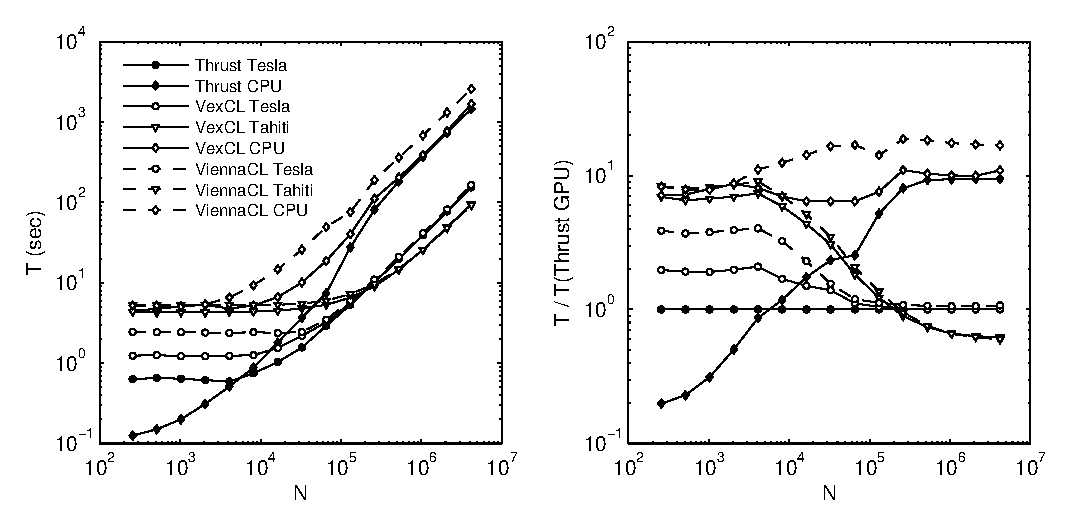
\includegraphics[width=\textwidth]{data/damped_oscillator/perfcmp}
    \end{center}
    \caption{Damped harmonic oscillator ensemble results.}
    \label{fig:damped:perf}
\end{figure}

\begin{figure}[p]
    \begin{center}
        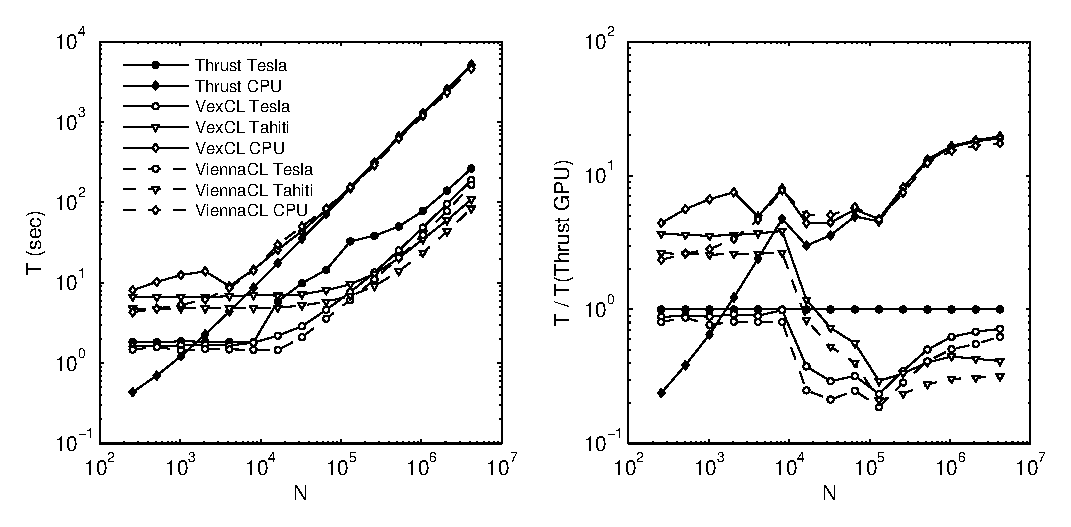
\includegraphics[width=\textwidth]{data/phase_oscillator_chain/perfcmp}
    \end{center}
    \caption{Coupled phase oscillator chain results.}
    \label{fig:phase:perf}
\end{figure}

\begin{figure}[p]
    \begin{center}
        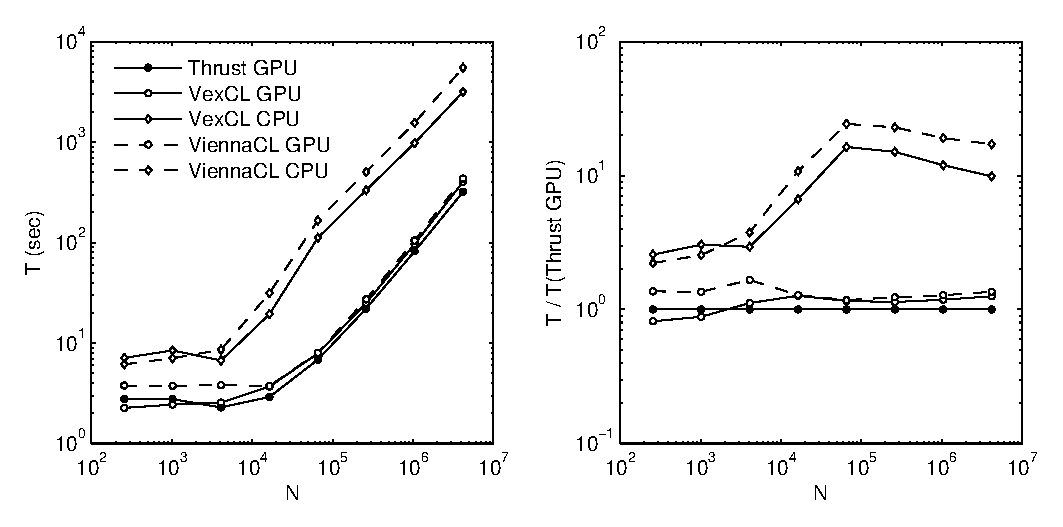
\includegraphics[width=\textwidth]{data/disordered_ham_lattice/perfcmp}
    \end{center}
    \caption{Disordered Hamiltonian lattice results.}
    \label{fig:lattice:perf}
\end{figure}

\begin{figure}[p]
    \begin{center}
        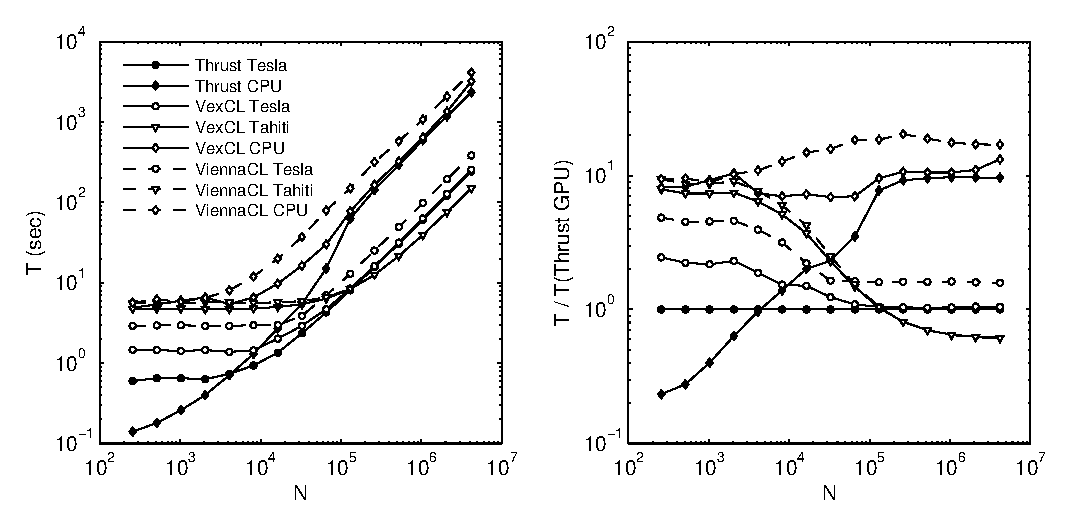
\includegraphics[width=\textwidth]{data/lorenz_ensemble/perfcmp}
    \end{center}
    \caption{Lorenz attractor ensemble results.}
    \label{fig:lorenz:perf}
\end{figure}

\begin{figure}[p]
    \begin{center}
        \subfigure[
        Damped harmonic oscillator ensemble.
	]{\label{fig:scaling:damped}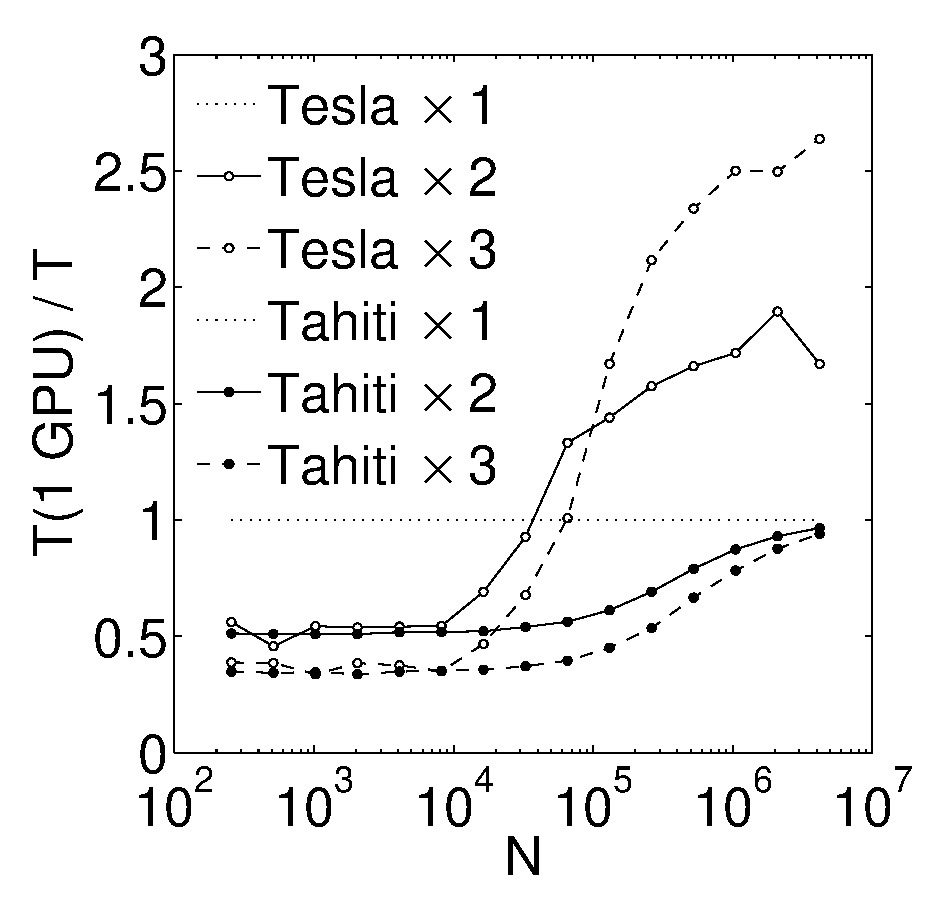
\includegraphics[width=0.45\textwidth]{data/damped_oscillator/scaling}}\quad
        \subfigure[
        Coupled phase oscillator chain.
        ]{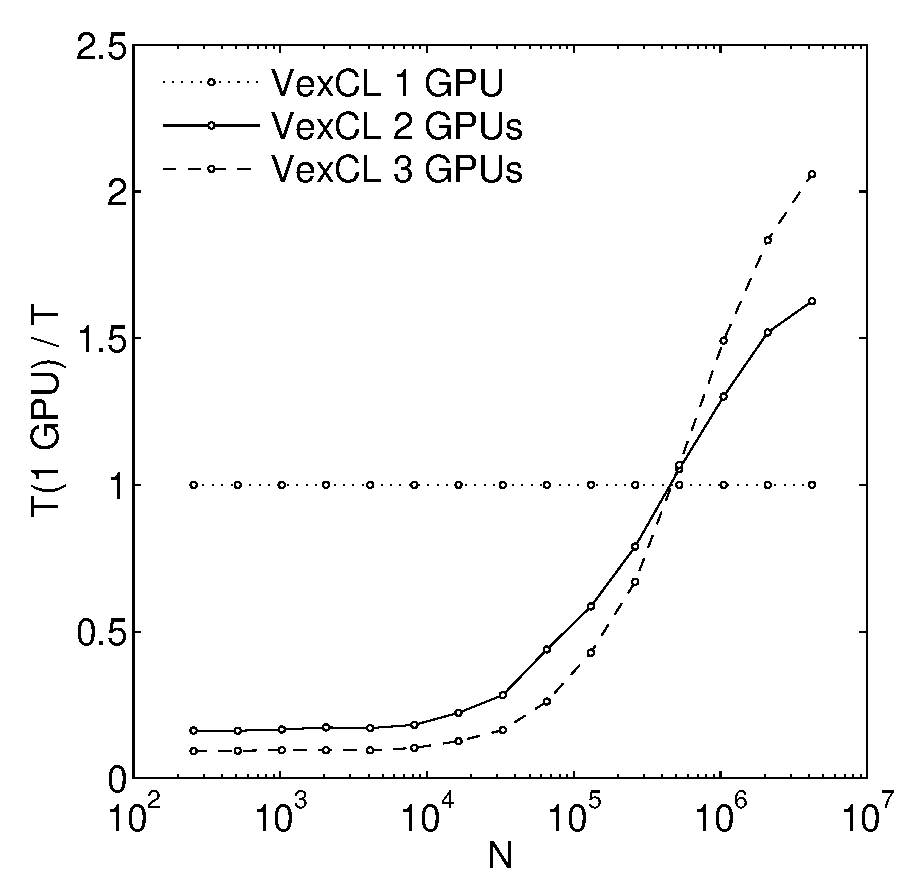
\includegraphics[width=0.45\textwidth]{data/phase_oscillator_chain/scaling}}\\
        \subfigure[
        Disordered Hamiltonian lattice.
        ]{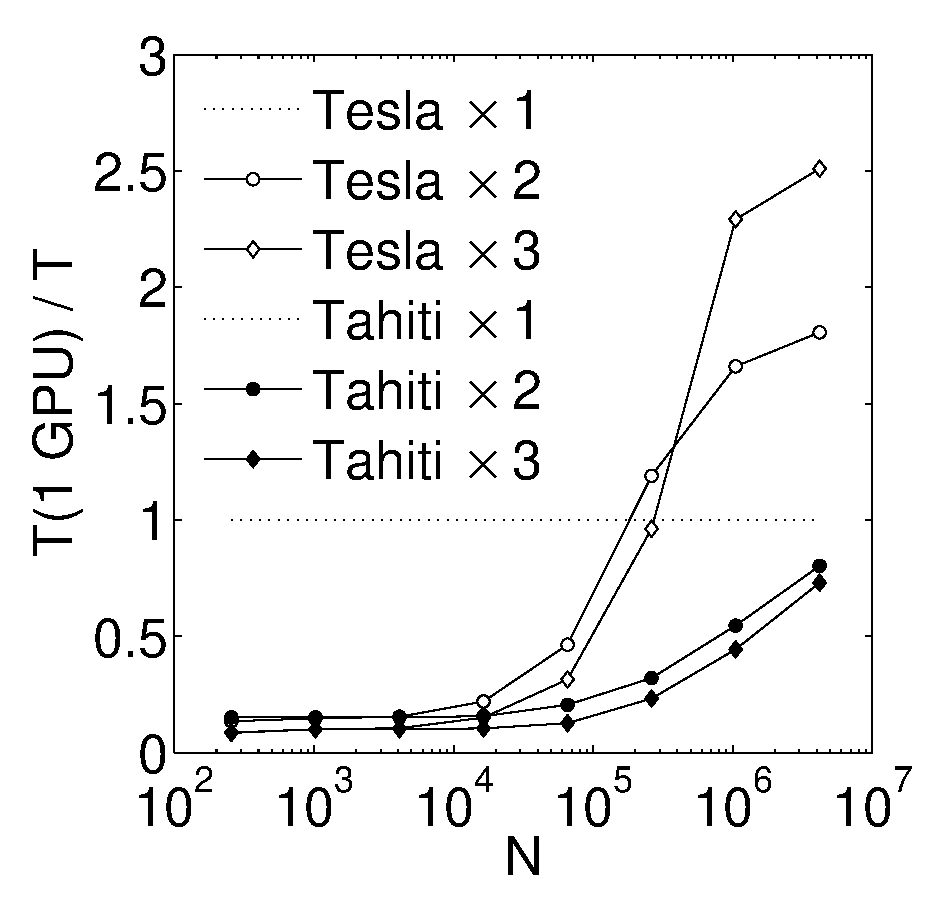
\includegraphics[width=0.45\textwidth]{data/disordered_ham_lattice/scaling}}\quad
        \subfigure[
        Lorenz attractor ensemble.
        ]{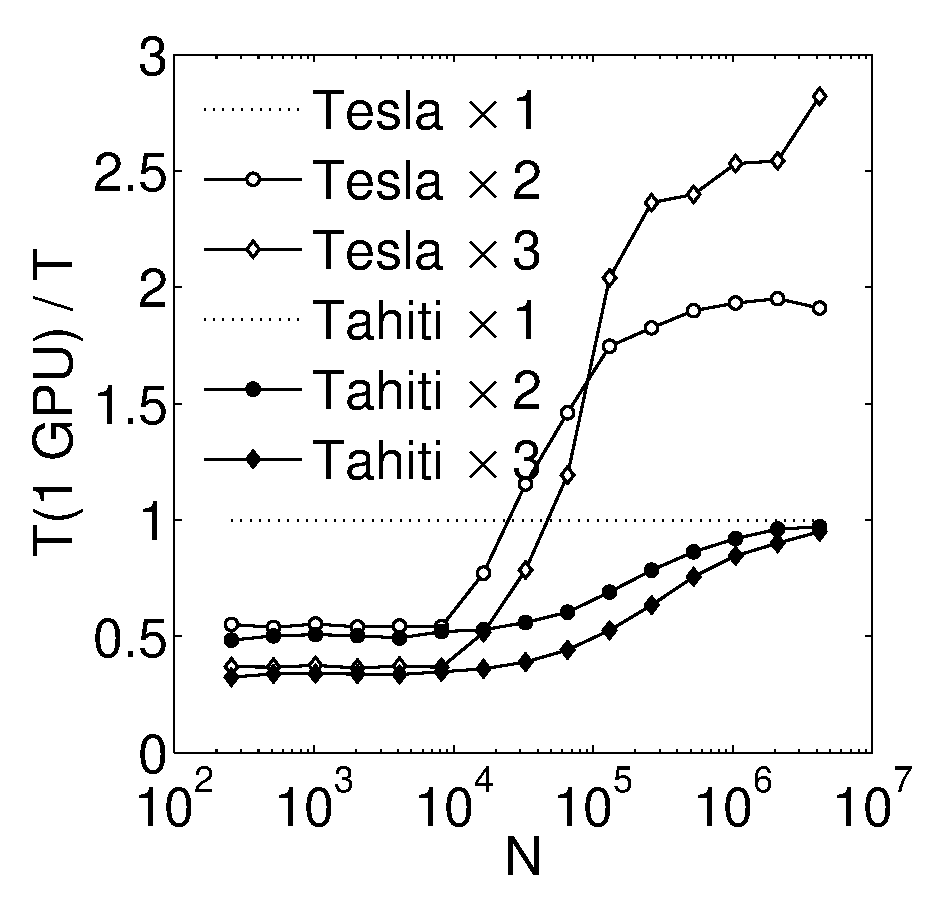
\includegraphics[width=0.45\textwidth]{data/lorenz_ensemble/scaling}}
    \end{center}
    \caption{VexCL scaling with multigpu computation.}
    \label{fig:scaling}
\end{figure}









%
% CONCLUSION
%
\section{Conclusion}

Performance-wise, there is almost no difference between various platforms and
libraries when those are run on the same hardware. As we have shown, various
computational problems may be solved effectively in terms of both human and
machine time with the help of modern high-level libraries.  There are some
differences in the programming interfaces of the libraries which may be crucial
for ones specific application.

Thrust is more low-level and its interface is very close to the C++ STL
library.  The OpenCL libraries we looked at demonstrated that they are able to
provide more convenient interface for a scientific programmer than a direct
implementation in CUDA or OpenCL.  VexCL has richer set of elementwise vector
operations, while ViennaCL has extensive set of sparse linear systems solvers,
which we did not discuss in this paper.

Regarding a comparison of CUDA versus OpenCL, we believe that OpenCL has a
major difference with respect to CUDA. Namely, it has a  much wider range of
supported hardware, which is only going to extend with time because it is an
open standard supported by major hardware producers. The other OpenCL advantage
that we did not explore in this paper is the ability to generate kernels
optimized for the problem at hand at runtime. We believe that this feature has
good potential, but we leave its in-depth discussion for the future work.  On
the other hand, this feature of OpenCL may be considered its drawback: runtime
kernel compilation adds certain overhead notable for smaller workloads as has
been shown in this paper.

% [DD]: OpenCL libraries showed excelent functional portability but not so good
% performance portability.

% [DD]: Some words about odeint generality that allowed us to run the set of
% experiments.



\section{Acknowledgments}

This work has been partially supported by RFBR grant No 12-07-0007. We also
would like to thank Gradient JSC\footnote{ \href{
http://www.gradient-geo.com/en }{ http://www.gradient-geo.com/en } } for the
kindly provided AMD hardware.


\bibliographystyle{siam}
\bibliography{ref}

\end{document}
% vim: set et
